\documentclass{article}
\usepackage{algorithm}
\usepackage{algpseudocodex}
\usepackage{graphicx}
\usepackage{amsmath}
\pagestyle{empty}
\title{CSEP521 : Applied Algorithms: Final}
\author{Karuna Sagar Krishna}

\begin{document}
    \maketitle

    \section*{Question 1}

    \subsection*{1a}
    \textbf{False}

    The question implicitly assumes that the min cut remains the same when the capacities of every edge is increased by 2. However, this is not always true as demonstrated by the graph below. Hence, as shown in the below graph, the max flow is not increased by 2 times the number of edges from $S$ to $T$ in $G$.

    Initially, the max flow was $x$ and the min cut was $S = \{s, v_0\}$ (remaining vertices are in $T$). Then we increased the capacities of each edge by 2, now the max flow is $x+3$ and the min cut is $S' = \{s\}$. Clearly, the min cut has changed and the new max flow is not increased by 2 times the number of edges from $S$ to $T$

    \begin{figure}[H]
        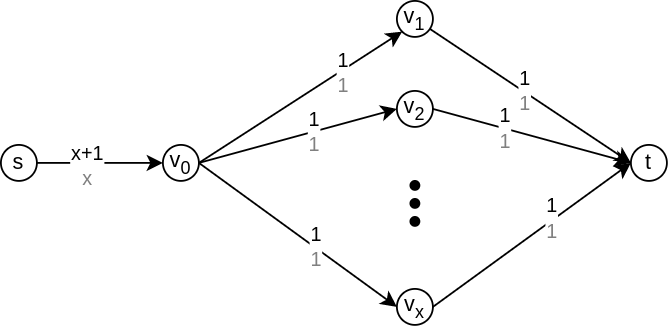
\includegraphics[width=1\textwidth]{maxflowIncreasedCapacity1.png}
    \end{figure}

    \begin{figure}[H]
        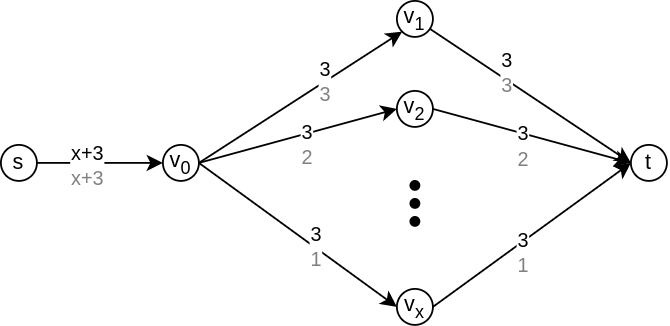
\includegraphics[width=1\textwidth]{maxflowIncreasedCapacity2.png}
    \end{figure}

    \subsection*{1b}
    \textbf{True}

    We could have a naive algorithm that iterates through all subsets of vertices checking to see if this subset covers all the edges and recording this subset if it has the minimum cardinality. There are $2^n$ subsets and each iteration takes $O(m) = O(n^2)$ time to verify if all edges are covered. Therefore, this algorithm takes $2^n + O(n^2) = 2^n$ time.

    \subsection*{1c}
    \textbf{True}

    We can compute $k = n/10$ in constant time. As clarified, we can assume that $k$ is an integer. Then the problem can be rephrased as find the $k$'th smallest number in a list of $n$ numbers, which we have solved in class in linear time.

    \subsection*{1d}
    \textbf{False}

    Applying master recurrence theorem, we get $\Theta(n^{\log_2 3})$ since $a > b^d$ i.e. $3 > 2^1$. Clearly, this does not grow the same as $\Theta(n^{\log_3 2})$

    \subsection*{1e}
    \textbf{True}

    Applying master recurrence theorem, we get $\Theta(n^2)$ since $a < b^d$ i.e. $12 < 4^2$

    \subsection*{1f}
    \textbf{False}

    As we proved in class, 3-SAT is NP complete problem. To solve any NP problem we can first spend polynomial time (by definition of NP complete) to reduce it to 3-SAT and then solve 3-SAT in linear time. However, the reduction is not necessarily linear hence the overall solution to any NP problem is not necessarily linear.

    \subsection*{1g}
    \textbf{False}

    In class, we discussed $EXP$ as a set of decision problems with runtime in the form $O(2^{f(n)})$ where $f(n)$ is some polynomial in input length $n$. However, there might be some decision problem with factorial complexity which grows faster than exponential functions and not part of $EXP$

    \subsection*{1h}
    \textbf{True}

    We've proved in class that every tree with $n$ vertices has exactly $n-1$ edges. Each edge contributes 2 to overall sum of degrees. So the sum of degrees across all vertices is $2(n-1)$, hence average degree per vertex is $\frac{2(n-1)}{n} = 2 - \frac{2}{n}$

    \subsection*{1i}
    \textbf{True}

    In class, we discussed why linear programs are powerful by showing that any boolean circuit can be represented as a linear program. Any instance of Program-SAT is a boolean circuit which can be converted to linear program. This conversion is mechanical and can be done in polynomial time by iterating through each line of the Program-SAT instance. Also, as we saw in class, computing the boolean circuit is equivalent to finding satisfying assignment to linear program constraints.

    \subsection*{1j}
    \textbf{True}

    Yes, as seen in class, linear programs can be solved in polynomial time using ellipsoid algorithm.

    \subsection*{1k}
    \textbf{True}

    The cut property of MST says that the minimum weight edge crossing any cut must be included in every MST. Say, $e = (u, v)$ and consider the cut formed by $\{u\}$ and $V - \{u\}$. Clearly, $e$ is the minimum weight edge crossing this cut and by cut property $e$ should be included in every MST.

    \subsection*{1l}
    \textbf{True}

    We could think of any linear program as finding the farthest point in the polytope defined by a set of inequality constraints. So if the linear program has an optimal solution, we can visualize this as a vertex on this polytope. Note, there could more than one vertex and even an edge that represents this optimal solution.

    \subsection*{1m}
    \textbf{False}

    Below is a counter example. Each edge in $G_3$ has capacity equal to the sum of the capacities of corresponding edge in $G_1$ and $G_2$ as indicated by the question. However, the max flow in $G_3$ is not the sum of max flow in $G_1$ and $G_2$

    \begin{figure}[H]
        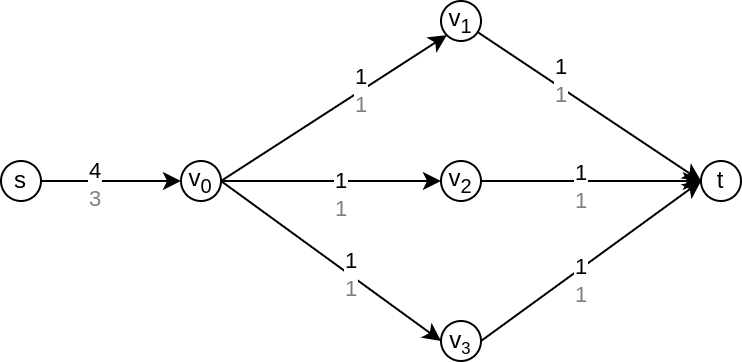
\includegraphics[width=1\textwidth]{maxflow1.png}
        \caption{$G_1$ has max flow of 3}
    \end{figure}

    \begin{figure}[H]
        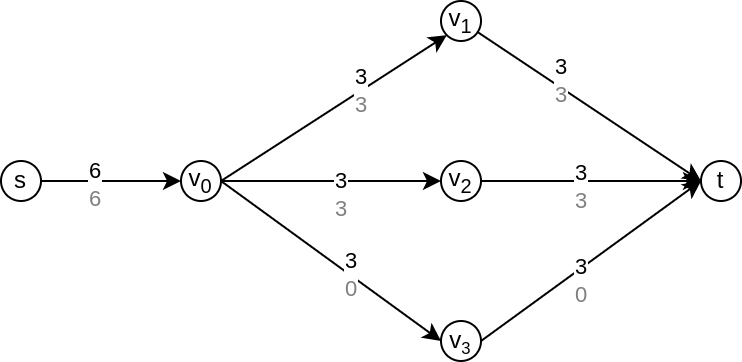
\includegraphics[width=1\textwidth]{maxflow2.png}
        \caption{$G_2$ has max flow of 6}
    \end{figure}

    \begin{figure}[H]
        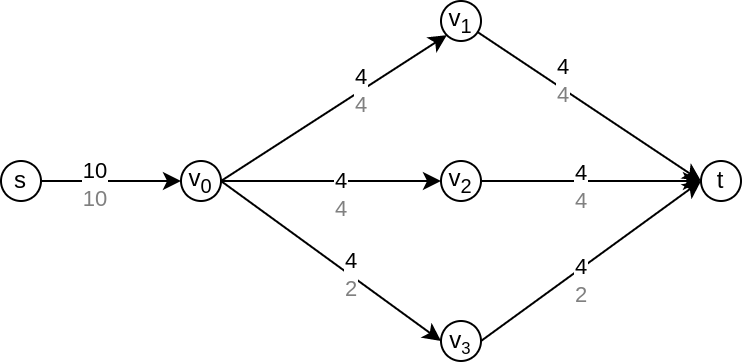
\includegraphics[width=1\textwidth]{maxflow3.png}
        \caption{$G_3$ has max flow of 10}
    \end{figure}

    \subsection*{1n}
    \textbf{True}

    We saw a greedy algorithm to find the vertex cover that is atmost twice as big as size of optimal cover. The greedy rule is to pick edge that is not covered by any vertex chosen for the cover so far. One way to implement this greedy algorithm is to iterate over edges, adding its endpoints to our vertex cover and then removing all other edges touching these endpoints. This would run in $O(n+m)$ as each edge and vertex is visited once.

    \subsection*{1o}
    \textbf{False}

    We've proved in class that, the max number of edge disjoint paths is equal to the max flow. The max flow is atmost the capacity of any cut. So it is not possible to have number of edge disjoint paths to exceed the min cut. Since the capacity of some cut (assuming unit capacity for all edges) $l$ is greater than or equal to min cut, it is not possible to have atleast $l$ edge disjoint paths.

    \subsection*{1p}
    \textbf{True}

    $f(x)$ is a decision problem to determine if $x$ is sum of squares. If we show this is in $NP$, then we can reduce this to 3-SAT in polynomial time since 3-SAT is NP complete. We then solve 3-SAT using the given polynomial time algorithm. Hence, $f(x)$ can be solved in polynomial time.

    To prove $f(x)$ is in $NP$, we provide the following certifier that runs in polynomial time. This certifier takes the input to the decision problem $x$ and certificate $y$ and $z$ which are integers. Note, valid certifiers would satisfy $|y| \le |x|$ and $|x| \le |x|$. The certifier performs two integer multiplications for which we learnt Karatsuba's algorithms which runs in polynomial time and one integer addition which takes linear time.

    \begin{algorithm}[H]
        \begin{algorithmic}
            \Procedure{SumOfSquaresCertifier}{$x, y, z$}
                \If{$y*y + z*z = x$}
                    \State \Return $True$
                \Else
                    \State \Return $False$
                \EndIf
            \EndProcedure
        \end{algorithmic}
    \end{algorithm}

    \subsection*{1q}
    \textbf{True}

    Bellman Ford algorithm can detect negative weight cycles. This takes $O((n+m)n)$ time. Since $m = O(n^2)$, we can say Bellman Ford takes $O((n+n^2)n) = O(n^3)$ time.

    \subsection*{1r}
    \textbf{True}

    Since both 3-SAT and vertex cover are NP complete, we can reduce vertex cover problem instances to 3-SAT in polynomial time $f(x)$. In this question, since we have a $2^{O(\log^2 n)}$ algorithm to solve 3-SAT, we can solve vertex cover in $2^{O(\log^2 n)} + f(x) = 2^{O(\log^2 n)}$ time.

    \subsection*{1s}
    \textbf{True}

    We saw Kruskal's algorithm run in $O(m \log n)$ time when implemented using union find data structure.

    \subsection*{1t}
    \textbf{True}

    Divide the $n \times n$ input matrix to form $k \times k$ matrix where each element is a matrix of size $\frac{n}{k} \times \frac{n}{k}$. We are given an algorithm that multiplies $k \times k$ matrices using $r$ multiplications and $k^2$ additions. Since each element of this $k \times k$ matrix is a subproblem of size $\frac{n}{k}$, we'll have $r$ multiplications of $\frac{n}{k} \times \frac{n}{k}$ matrices and $k^2$ additions of $\frac{n}{k} \times \frac{n}{k}$ matrices. Thus running time is $T(n) = rT(\frac{n}{k}) + k^2 (\frac{n}{k})^2$, which can be simplified as $T(n) = rT(\frac{n}{k}) + n^2$. We are also told, $3 > \log_k r > 2$ which can be rewritten as $k^3 > r > k^2$. Applying master recurrence theorem, we get $T(n) = \Theta(n^{\log_k r})$ since $a > b^d$ i.e. $r > k^2$. Hence, we can multiply $n \times n$ matrices in $O(n^{\log_k r})$

    \section*{Question 2}

    \subsection*{Idea}
    If all edges have the same cost, it doesn't matter the order in which we pick the edges. So every spanning tree is a MST. BFS can find a breadth first spanning tree in $O(n+m)$ time.
    
    However, in the question we have a graph $G_0 = (V_0, E_0)$ whose edges have cost $\in \{1, 2, 3\}$. If we were to apply Kruskal's algorithm, we would have sorted the edges and then picked edges in this sorted order that don't form cycle. Clearly, we would have processed all edges with cost 1 and then processed all edges with cost 2 and so on. Also, Kruskal's would ignore edges that connect vertices in the same components to avoid cycles in spanning tree. So, consider a subgraph $G_1 = (V_1, E_1)$, where $V_1 = V_0$ and $E_1 = \{e \in E_0 : c(e) = 1\}$ i.e. $E_1$ only contains edges of $G_0$ with cost 1. Notice, $G_1$ is a graph with all edges having the same cost, hence we can run BFS to find a spanning tree. $G_1$ might be disconnected though $G_0$ is connected, hence BFS is run on each connected component of $G_1$. This produces a forest of spanning trees. Next, we create subgraph $G_2 = (V_2, E_2)$, where each vertex in $V_2$ represents the connected component in $G_1$ and $E_2 = \{e \in E_0 : c(e) = 2 \land \text{$e$ connects different components in $G_1$}\}$. Since all edges of $G_2$ have the same cost, we can run BFS again yielding again a forest of spanning trees. Similarly, we repeat this i.e create $G_3$ and run BFS. Since $G_0$ was connected, $G_3$ would be connected since it has encodes all the edges in $G_0$ since we constructed $G_3$ from $G_2$ which was inturn constructed from $G_1$ which was inturn constructed from $G_0$. So BFS on $G_3$ should return a single spanning tree and this would the MST of $G_0$.
    
    \subsection*{Algorithm}
        \begin{algorithm}[H]
            \begin{algorithmic}
                \Procedure{123MST}{$V_0, E_0$}
                    \For{$v \in V_0$}
                        \State $label_0[v] = v$
                    \EndFor

                    \For{$i \in \{1, 2, 3\}$}
                        \For{$v \in V_{i-1}$}
                            \State $V_i = V_i \cup \{label_{i-1}[v]\}$
                        \EndFor

                        \For{$(u, v) \in E_0$}
                            \If{$cost(u, v) = i \land IsSameComponent(u, v, i-1) = False$}
                                \State $u' = FindComponentLabel(u, i-1)$
                                \State $v' = FindComponentLabel(v, i-1)$
                                \State $o_i[(u', v')] = (u, v)$
                                \State $E_i = E_i \cup \{(u', v')\}$
                            \EndIf
                        \EndFor

                        \State $parent_i, label_i = BFS(V_i, E_i)$

                        \For{$v \in V_i$}
                            \If{$parent_i[v] \ne v$}
                                \State $e = (v, parent_i[v])$
                                \State $T = T \cup o_i[e]$
                            \EndIf
                        \EndFor
                    \EndFor

                    \State \Return $T$
                \EndProcedure

                \Procedure{FindComponentLabel}{$v, k$}
                    \For{$j \in \{0 \dots k\}$}
                        \State $v = label_j[v]$
                    \EndFor

                    \State \Return $v$
                \EndProcedure

                \Procedure{IsSameComponent}{$u, v, k$}
                    \For{$j \in \{0 \dots k\}$}
                        \If{$label_j[u] = label_j[v]$}
                            \State \Return $True$
                        \EndIf
                        \State $u = label_j[u]$
                        \State $v = label_j[v]$
                    \EndFor

                    \State \Return $False$
                \EndProcedure

                \Procedure{BFS}{$V, E$}
                    \For{$s \in V$}
                        \State $discovered[s] = False$
                    \EndFor

                    \For{$s \in V$}
                        \If{$discovered[s] = False$}
                            \State $discovered[s] = True$
                            \State $label[s] = s$
                            \State $parent[s] = s$

                            \State $queue.add(s)$
                            \While{$!queue.empty()$}
                                \State $u = queue.remove()$
                                \For{$(u, v) \in E$}
                                    \If{$disovered[v] = False$}
                                        \State $discovered[v] = True$
                                        \State $label[v] = s$
                                        \State $parent[v] = u$
                                        \State $queue.add(v)$
                                    \EndIf
                                \EndFor
                            \EndWhile
                        \EndIf
                    \EndFor

                    \State \Return $parent, label$
                \EndProcedure
            \end{algorithmic}
        \end{algorithm}

    \subsection*{Correctness}
    $123MST$ takes in the input graph $G_0 = (V_0, E_0)$. Labels represent the connected component that the vertex belongs to. We begin by labelling the vertices of $V_0$ such that each vertex is a connected component by itself since there is no edges in the MST found so far.

    Next, we construct subgraph $G_i = (V_i, E_i)$. $V_i$ contains a vertex for each connected component in the previous subgraph $G_{i-1}$. $E_i$ contains a edge from original graph $G_0$ whose cost is $i$ and connects two different connected component in $G_{i-1}$. Essentially, we shrink a connected component from $G_{i-1}$ to form a single vertex in $G_i$ and merge the edges of cost $i$ between these connected components. When we merge the original edges from $E_0$ in $G_i$, we lose the information about the original edge needed to build MST. Since all of these original edges getting merged are of the same cost and it doesn't matter which of these edges are part of MST, we need to track just one of them in $o_i$. In other words, for each edge in $G_i$ we track one of the original edge in $G_0$.
    
    We could have used union find data structure to track the connected components, however, this would introduce an additional $O(\log n)$ time complexity which can be avoided. So instead, we keep track of the component labels in $label_i$ for each subgraph $G_i$. Note, $label_i[v]$ represents the connected component that a vertex $v$ in subgraph $G_i$ belongs to. Also note that, $label_{i-1}[v]$ is a vertex in subgraph $G_i$. $IsSameComponent(u, v, i)$ is invoked to determine if an edge $(u, v) \in G_0$ connects different connected components in $G_i$. $IsSameComponent$ first checks the labels of both the edge endpoints in $G_0$, if the labels are equal, then clearly these endpoints belong to the same connected component. Then the endpoints are replaced with the corresponding labels in $G_0$ since this represents a vertex in $V_1$. The above check is repeated in $G_1$ and this process continues until we have verified the labels in each of the previous subgraphs. Hence, $IsSameComponent$ is correct since we have verified the connected component label for each of the previous graphs in order. $FindComponentLabel(v, i)$ is used to find the connected component label for vertex $v \in G_0$ in subgraph $G_i$. This is achieved by looking up the connected component label starting at $G_0$ and then looking up this value in $G_1$ and so on.

    Based on above, $123MST$ correctly constructs the subgraph $G_i$. Also note, subgraphs $G_i$ could be disconnected since we are only considering edges of certain cost. Specifically, $G_1$ only includes edges of cost 1, $G_2$ is constructed on top of connected components from $G_1$ using edges of cost 2 and finally $G_3$ is constructed on top of connected components from $G_2$ using edges of cost 3. This implies that though $G_1$, $G_2$ could be disconnected, $G_3$ is connected because it has considered all the edges of original graph $G_0$ and $G_0$ is connected.
    
    We then call $BFS$ on subgraph $G_i$. $BFS(V, E)$ is straightforward algorithm that we have proved in class. This handles the case when the given graph is disconnected. It labels vertices as it discovers them with the first starting vertex used for this discovery. In other words, vertices are labelled with the root of the breadth first tree. This $label$ information is used in subsequent iterations of $123MST$ as described above. $BFS$ also captures the parent vertex used for discovery. We use $parent$ information to grow the tree $T$ by iterating over the edges in breadth first tree and adding the corresponding original edge in $G_0$ that was captured in $o_i$ as explained above. After processing $G_1$ and $G_2$, $T$ would be a forest of trees containing all the vertices in $G_0$. $G_3$ is connected and hence there is only one connected component. So after processing $G_3$, $T$ would be a connected tree and spanning all the vertices in $G_0$. Finally, since we considered edges connecting different components in the increasing order of their cost (cut principle), $T$ is a minimum spanning tree.

    \subsection*{Analysis}
    $IsSameComponent(u, v, i)$ runs in $O(1)$. There are only 3 different edge costs and hence only 3 different subgraphs. So the for loop in $IsSameComponent$ can loop for a maximum of 3 times each iteration costing $O(1)$. Similarly, $FindComponentLabel$ also runs in $O(1)$. And $BFS$ takes $O(n+m)$ as proved in class.
    
    $V_i$ is atmost the same size as $V_0$ because we cannot have more number of connected components than the number of vertices in the original graph. Similarly, $E_i$ is atmost the same size as $E_0$ because we are only considering edges in $E_0$ and not introducing any new ones. Given, this $123MST$ takes $O(n) + 3[O(n) + O(m) + O(n+m) + O(n)] = O(n+m)$

    \section*{Question 3}

    \subsection*{Idea}
    The FFT algorithm is used to multiply two polynomials of degree $n$. In class, we assumed that $n$ is power of 2 (if not, we padded with zero coefficients). We then converted the polynomial from coefficient form to point value form, performed point-wise multiplication and then converted back from point value form to coefficient form. The main runtime complexity concern was regarding the conversion between the two forms (evaluation and interpolation).

    The FFT algorithm used 2 main ideas to expedite the conversion. First, we broke up the polynomial of degree $n$ into 2 smaller polynomials of degree $n/2$ each. Second, we used $n$ complex $n^{th}$ root of unity since these had a special property that when squared there were repetitions which allowed us to compute the smaller polynomial on the half the points.

    We need to modify these 2 main ideas i.e. break up the polynomial into 3 smaller polynomial of degree $n/3$ each and use the complex roots of unity to prove that special property holds when we cube them.
    
    \subsection*{Algorithm}
        \begin{algorithm}[H]
            \begin{algorithmic}
                \Procedure{PolynomialMultiply}{$p, q$}
                    \State \text{$p$ and $q$ are polynomials of degree $n$}
                    \State \text{Goal is to compute $r = p*q$ of degree $2n$}
                    \State \text{Set $m$ to be a power of 3, $m > 2n$} \\

                    \State $pv = Evaluate(p, m)$
                    \State \text{This computes $p(\omega^0), p(\omega^1), \dots p(\omega^m)$}
                    \State $qv = Evaluate(q, m)$
                    \State \text{This computes $q(\omega^0), q(\omega^1), \dots q(\omega^m)$} \\

                    \State $rv = PointWiseMultiple(pv, qv, m)$
                    \State \text{This computes $r(\omega^0), r(\omega^1), \dots r(\omega^m)$ using $r(\omega^i) = p(\omega^i)*q(\omega^i)$} \\

                    \State $r = Interpolate(rv, m)$
                    \State \Return $r$
                \EndProcedure

                \Procedure{Evaluate}{$a, m$}
                    \State \text{Goal is to evaluate $a(x)$ of degree $m$ at $m$ complex $m^{th}$ root of unity}
                    \State \text{i.e. evaluate $a(\omega^0), a(\omega^1), a(\omega^2), \dots a(\omega^{m-1})$} \\

                    \State \text{Polynomial $a(x) = a_0x^0 + a_1x^1 + \dots a_mx^m$ can be rewritten as}
                    \State \text{$a(x) = b_0(x^3) + xb_1(x^3) + x^2b_2(x^3)$ where}
                    \State \text{$b_0(y) = a_0y^0 + a_3y^1 + a_6y^2 + a_9y^3 + \dots $}
                    \State \text{$b_1(y) = a_1y^0 + a_4y^1 + a_7y^2 + a_{10}y^3 + \dots $}
                    \State \text{$b_2(y) = a_2y^0 + a_5y^1 + a_8y^2 + a_{11}y^3 + \dots $} \\

                    \State \text{Recursively evaluate}
                    \State \text{$b_0(\omega^0), b_0(\omega^3), b_0(\omega^6), \dots b_0(\omega^{3(m-1)})$ using $Evaluate(b_0, m/3)$,}
                    \State \text{$b_1(\omega^0), b_1(\omega^3), b_1(\omega^6), \dots b_1(\omega^{3(m-1)})$ using $Evaluate(b_1, m/3)$,}
                    \State \text{$b_2(\omega^0), b_2(\omega^3), b_2(\omega^6), \dots b_2(\omega^{3(m-1)})$ using $Evaluate(b_2, m/3)$}
                    \State \text{Note, $(\omega^k)^3 = (\omega^{k+m/3})^3 = (\omega^{k+2m/3})^3$}
                    \State \text{Hence we are evaluating $b_0$, $b_1$ and $b_2$ at $m/3$ points}\\

                    \State \text{Compute and return $a(\omega^0), a(\omega^1), a(\omega^2), \dots a(\omega^{m-1})$ as}
                    \State \text{$a(\omega^i) = b_0(\omega^{3i}) + \omega^i b_1(\omega^{3i}) + \omega^{2i} b_2(\omega^{3i})$}
                \EndProcedure

                \Procedure{Interpolate}{$rv, m$}
                    \State \text{Goal is to compute $r(x)$ given $m$ values of $r(x)$ as $rv$}
                    \State \text{$r(x) = r_0x^0 + r_1x^1 + \dots r_mx^m$} \\

                    \State \text{Let $q(x) = r(\omega^0)x^0 + r(\omega^1)x^1 + r(\omega^2)x^2 \dots r(\omega^{m-1})x^{m-1}$}
                    \State \text{Compute $q(\omega^0), q(\omega^1), \dots q(\omega^{m-1})$ using $Evaluate(q, m)$} \\

                    \For{$i \in \{0 \dots m-1\}$}
                        \State \text{Set $r_i = \frac{q(\omega^{m-i})}{m}$}
                    \EndFor \\

                    \State \Return $r$
                \EndProcedure

                \Procedure{PointWiseMultiple}{$pv, qv, m$}
                    \For{$i \in \{0 \dots m-1\}$}
                        \State $rv_i = pv_i * qv_i$
                    \EndFor

                    \State \Return $rv$
                \EndProcedure
            \end{algorithmic}
        \end{algorithm}

    \subsection*{Correctness}
    The original input polynomials ($p$ and $q$) are of degree $n$. We add higher degree zero coefficients to convert it into polynomial of degree $m$, where $m$ is chosen such that it is power of 3 and $m > 2n$. Since the product of two $n$ degree polynomials is $2n$, we need to evaluate and interpolate $2n$ points.

    $Evaluate(a, m)$ recursively evaluates the polynomial $a(x)$ of degree $m$ at $m$ complex $m^{th}$ roots of unity. To do so, we need 2 things:
    \begin{enumerate}
        \item break the input polynomial of degree $m$ into smaller polynomial in terms of degree. Specifically, we want 3 smaller polynomials each of degree $m/3$
        \item the smaller polynomials are evaluated at $m/3$ points
    \end{enumerate}

    Polynomial $a(x) = a_0x^0 + a_1x^1 + \dots a_mx^m$ is broken into 3 smaller polynomials $b_0(x)$, $b_1(x)$ and $b_2(x)$ each of degree $m/3$. $b_0(x)$ contains coefficients of the form $a_{3r}$, $b_1(x)$ contains coefficients of the form $a_{3r+1}$ and $b_2(x)$ contains coefficients of the form $a_{3r+2}$. This allows us to rewrite $a(x)$ as $b_0(x^3) + xb_1(x^3) + x^2b_2(x^3)$.

    We learnt in class that when we square the $m$ complex $m^{th}$ roots of unity, we get $m/2$ complex ${m/2}^{th}$ roots of unity. The $k^{th}$ complex $m^{th}$ root of unity is $\omega_m^k = e^{\frac{2\pi ik}{m}}$. When we cube this we get
    \begin{align*}
        (\omega_m^k)^3  & = (e^{\frac{2\pi ik}{m}})^3 \\
                        & = e^{\frac{6\pi ik}{m}} \\
    \end{align*}
    Also,
    \begin{align*}
        (\omega_m^k)^3  & = (e^{\frac{2\pi ik}{m}})^3 \\
                        & = e^{\frac{2\pi ik}{m/3}} \\
                        & = \omega_{m/3}^k \\
    \end{align*}

    Now, consider, cubing $\omega_m^{k+m/3}$ and $\omega_m^{k+2m/3}$ we get the following. Note, $e^{2\pi i} = 1$ and $e^{4\pi i} = 1$
    \begin{align*}
        (\omega_m^{k+m/3})^3    & = (e^{\frac{2\pi i(k+m/3)}{m}})^3 \\
                                & = e^{\frac{2\pi i(3k+m)}{m}} \\
                                & = e^{\frac{6\pi ik + 2\pi im}{m}} \\
                                & = e^{\frac{6\pi ik}{m}} e^{\frac{2\pi im}{m}} \\
                                & = (\omega_m^k)^3 e^{2\pi i} \\
                                & = (\omega_m^k)^3 \\
    \end{align*}

    \begin{align*}
        (\omega_m^{k+2m/3})^3   & = (e^{\frac{2\pi i(k+2m/3)}{m}})^3 \\
                                & = e^{\frac{2\pi i(3k+2m)}{m}} \\
                                & = e^{\frac{6\pi ik + 4\pi im}{m}} \\
                                & = e^{\frac{6\pi ik}{m}} e^{\frac{4\pi im}{m}} \\
                                & = (\omega_m^k)^3 e^{4\pi i} \\
                                & = (\omega_m^k)^3 \\
    \end{align*}

    Hence, the cube of $\omega_m^k$, $\omega_m^{k+m/3}$ and $\omega_m^{k+2m/3}$ are equal and equal to $\omega_{m/3}^k$. In other words, when we cube all the $m$ complex $m^{th}$ roots of unity we get $m/3$ complex ${m/3}^{th}$ roots of unity. Notice, to evaluate $a(x)$ at $m$ complex $m^{th}$ roots of unity we need to evaluate $b_0(x^3)$, $b_1(x^3)$ and $b_2(x^3)$. Hence, we only need to evaluate $b_0(x)$ at $m/3$ complex ${m/3}^{th}$ roots of unity and similarly for $b_1(x)$ and $b_2(x)$. We already saw that $b_0(x)$, $b_1(x)$ and $b_2(x)$ are of degree $n/3$. Hence, the subproblems of evaluating $b_0$, $b_1$ and $b_2$ can be done recursively. Finally, the results from subproblems are put together to evaluate $a(x)$. This proves the correctness of $Evaluate(a, m)$

    $Interpolate(rv, m)$ takes in the point value form of a polynomial $r(x)$ of degree $m$ and returns the coefficient form. Specifically, $rv$ is a vector containing the evaluation of a polynomial $r(x)$ at $m$ complex $m^{th}$ roots of unity. As we saw in class, we create a new polynomial $q(x)$ using the provided input values ($rv$) as coefficients. We then evaluate this polynomial to determine the coefficients of $r(x)$. At a high level, there is no change in this algorithm, except that we call $Evaluate$ which breaks recursively evaluates the polynomial using 3 subproblems instead of 2 as seen in class. We've proved above the correctness of $Evaluate$, combining this with the proof we saw in class, we can conclude that $Interpolate$ is correct.

    $PointWiseMultiple$ takes in the point value form of two polynomials $p(x)$ and $q(x)$. Specifically, $pv$ and $qv$ are vectors containing the evaluation of a polynomial $p(x)$ and $q(x)$ respectively at $m$ complex $m^{th}$ roots of unity. As we saw in class, in point value form, the product of two polynomials at $k$ i.e. $(k, p(k))$ and $(k, q(k))$ is $(k, p(k)*q(k))$. $PointWiseMultiple$ iterates through each point and calculates this product.

    Finally, $PolynomialMultiply(p, q)$ is similar to the FFT outline we saw in class. The main difference is that we set $m$ to be a power of 3 such that $m > 2n$ and we call $Evaluate$ and $Interpolate$ discussed above which recursively computes using 3 subproblems instead of two. As shown above, $Evaluate$, $Interpolate$ and $PointWiseMultiple$ are correct. Combining this with the proof we saw in class, we can conclude that $PolynomialMultiply$ is correct.

    \subsection*{Analysis}
    $Evaluate$ breaks the input problem into 3 subproblems of equal size in linear time. It then computes the results for the input problem using the results of the subproblem in linear time. Hence, we get the recurrence equation $T(n) = 3T(n/3) + O(n)$. Using master recurrence theorem, we get $T(n) = \Theta(n \log n)$ since $a = b^d$ i.e. $3 = 3^1$.

    $Interpolate$ constructs polynomial $q(x)$ in linear time. It then calls $Evaluate$ which takes $O(n \log n)$ as shown above. And finally, it computes the coefficients of $r(x)$ in linear time. Hence, $Interpolate$ takes $O(n) + O(n \log n) + O(n) = O(n \log n)$ time.

    $PointWiseMultiple$ runs in $O(n)$ time.

    $PolynomialMultiply$ calls $Evaluate$ twice (once for each input polynomial) and calls $PointWiseMultiple$, $Interpolate$ once. Hence, $PolynomialMultiply$ runs in $O(n \log n) + O(n \log n) + O(n) + O(n \log n) = O(n \log n)$ time. Note, though we modified the algorithm discussed in class, the time complexity remains the same.

    \section*{Question 4}

    \subsection*{Idea}
    We'll use the same recursive algorithm for selecting $k^{th}$ smallest number that we saw in class, except that instead of splitting into $n/5$ sets of size 5 we'll split into $n/4$ sets of size 4. We'll perform similar time complexity analysis as we did in class.
    
    \subsection*{Algorithm}
        \begin{algorithm}[H]
            \begin{algorithmic}
                \Procedure{Select}{$A, k$}
                    \State \text{Goal is to find $k^{th}$ element in array $A$ of length $n$} \\

                    \State \text{Partition numbers into sets of 4}
                    \State \text{Sort each set}
                    \State \text{In each set, find the median which is the average of middle two elements}
                    \State \text{Recursively find the median of medians from each set, lets call it $w$} \\

                    \State \text{Partition the array $A$ around $w$}
                    \State \text{$S_L = \{x_i | x_i < w \land x_i \in A\}$}
                    \State \text{$S_E = \{x_i | x_i = w \land x_i \in A\}$}
                    \State \text{$S_G = \{x_i | x_i > w \land x_i \in A\}$} \\

                    \If{$k \le |S_L|$}
                        \State \Return $Select(S_L, k)$
                    \ElsIf{$k \le |S_L| + |S_E|$}
                        \State \Return $w$
                    \Else
                        \State \Return $Select(S_G, k - |S_L| - |S_E|)$
                    \EndIf
                \EndProcedure
            \end{algorithmic}
        \end{algorithm}

    \subsection*{Correctness}
    The algorithm $Select(A, k)$ is mostly the same as we saw in class. The main change is that we split the array $A$ into sets of size 4. This implies that $n$ should be a power of 4. Though not shown in the above algorithm, if $n$ is not a power of 4, on each recursive call we can massage $A$ and $k$ to make $n$ divisible by 4. Specifically, we'll find the minimum in the array in linear time and adjust $k$ accordingly. We repeat this until $n$ is divisible by 4, hence we'll be repeating this upto 3 times.

    Each set is sorted and the set median is computed in constant time. As suggested in the question, the median of 4 element set is computed as average of the middle two elements. Note that there are $n/4$ sets, hence it takes linear time to sort and compute the set medians over all sets. Unlike what we saw in class, the set medians need not belong to $A$; if the middle two elements are different, then set median doesn't belong to $A$ but if they are equal, then set median belongs to $A$. We then compute $w$ as median of set medians by recursively calling $Select$ on the array of set medians to find the middle i.e. $n/8^{th}$ element. As we saw with set medians, $w$ may not exist in the original array $A$.

    Based on $w$, we partition $A$ into $S_L$ containing elements less than $w$, $S_E$ containing elements equal to $w$ and $S_G$ containing elements greater than $w$. If $k$ is less than $|S_L|$, then clearly we need to find $k^{th}$ element in $S_L$. Otherwise, if $k$ is less than $|S_L| + |S_E|$, then we already know that $k^{th}$ element is in $S_E$ and since $S_E$ only contains elements of $A$ that are equal to $w$, we can say that the  $k^{th}$ element is $w$. Otherwise,  $k^{th}$ element of $A$ is in $S_G$; we need to adjust $k$ as $k - |S_L|  - |S_E|$ so that we correctly find the $k^{th}$ element of $A$ using recursion. This proves the correctness of $Select$.

    \subsection*{Analysis}
    \begin{figure}[H]
        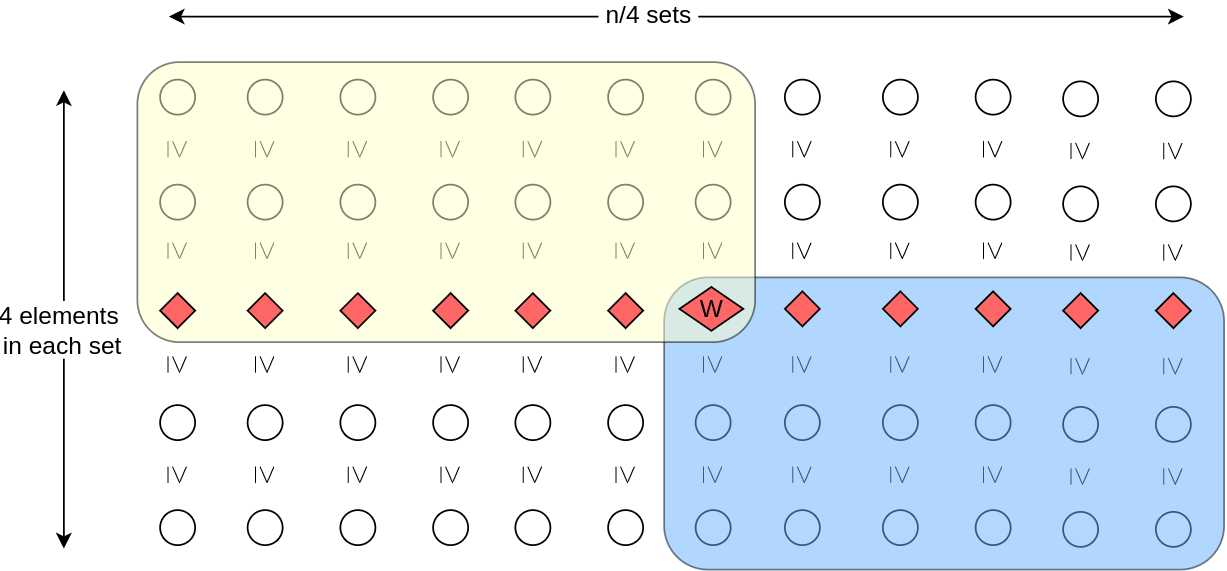
\includegraphics[width=1\textwidth]{selectkth.png}
    \end{figure}

    The above diagram shows $n/4$ sets of size 4. Elements (shown as circles) within a set are sorted with larger element at the top of smaller elements. Since each set contains 4 elements, the median is the average of middle two elements and this is shown as red diamond in the diagram. Note, the median is shown in red diamond since it may not be part of the original array $A$, it is shown for reasoning the correctness and analysis only. The median of all set medians is shown as red diamond and marked as $w$. Again, $w$ may not exist in the array $A$, further if $n/4$ is even, then $w$ is itself the average of middle two set medians. The sets to the left of $w$ have set medians greater than or equal to $w$, while the sets to the right of $w$ have set medians less than or equal to $w$. The relative ordering of the sets itself doesn't matter. Hence, the yellow region contains elements that are greater than or equal to $w$, while the blue region contains elements that are less than or equal to $w$. Elements outside the yellow and blue region can be lesser than or greater than $w$.
    
    Assume that set medians don't exist in $A$ i.e. the middle two elements of each set is different.We'll assume this so that we evaluate the worst case for this algorithm. Since $w$ is median of set medians, there are atmost $n/8$ sets to the left of it and atmost $n/8$ sets to the right of it. The yellow region contains atmost $n/4$ elements since in each set to left of $w$ there are exactly 2 elements that are greater than or equal to $w$. Similarly, the blue region contains atmost $n/4$ elements. We can say that there are atleast $n/4$ elements greater than or equal to $w$ and similarly there are atleast $n/4$ elements lesser than or equal to $w$. We can also say, there are atmost $n-n/4 = 3n/4$ elements greater than or equal to $w$ and similarly there are atmost $n-n/4 = 3n/4$ elements less than or equal to $w$. Hence, $|S_G| \le 3n/4$ and $|S_L| \le 3n/4$.

    Lets say, $T(n)$ is the time taken by $Select$ to find the $k^{th}$ element among $n$ elements of array. Dividing elements of $A$ into $n/4$ sets can be done in linear time. Sorting and computing the set median takes linear time as discussed above. The median of set medians is computed recursively on array of size $n/4$. Partitioning $A$ into $S_L$, $S_E$ and $S_G$ can be done in linear time. And finally, we perform atmost one recursive call on either $S_L$ or $S_G$ and as shown above each of these arrays are of size $3n/4$. So overall, it takes $T(n) = O(n) + O(n) + T(n/4) + O(n) + T(3n/4)$ or $T(n) = T(n/4) + T(3n/4) + O(n)$. As seen in class, recurrence for the form $T(n) = T(\beta n) + T(\gamma n) + n$ can be solved as $T(n) = n \sum_{i=0}^{i=\log n} (\beta + \gamma)^i$. So, $T(n) = n \sum_{i=0}^{i=\log n} (1/4 + 3/4)^i$. Hence, $Select$ takes $O(n \log n)$ time. If we assumed that all set medians could exist in $A$ because the middle two elements of the sets are equal, then $Select$ would take linear time. This is because we would have atleast $3n/8$ elements greater than or equal and less than or equal to $w$. And, $|S_L|$ and $|S_G|$ would be atmost $5n/8$ leading to a recurrence $T(n) = T(n/4) + T(5n/8) + O(n)$ which solve to give $O(n)$ time.

    Hence, the upper bound of $Select$ is $O(n \log n)$.

\end{document}
 